\newgeometry{
    a4paper,
    top=24mm,
    bottom=28mm,
    left=39mm,
    right=39mm,
    heightrounded
}
\partpage{Magnetostatica}
\restoregeometry

\chapter{Corrente elettrica}

I materiali conduttori solidi sono costituiti da un reticolo cristallino spaziale ai cui vertici si trovano gli ioni positivi (atomi che hanno ceduto uno o più elettroni) e al cui interno si muovono gli elettroni liberi, i portatori mobili di carica. \\ 

Se si mettono a contatto due conduttori $C_1$ e $C_2$ isolati a potenziali elettrostatici $V_1$ e $V_2$ diversi, si raggiunge una condizione di equilibrio in cui entrambi i conduttori si portano allo stesso potenziale elettrostatico $V$. Nel processo un certo numero di elettroni passa dal conduttore a potenziale minore a quello a potenziale maggiore, sotto l'azione del campo elettrico $\mathbf{E}$ dovuto alla differenza di potenziale $V_2 - V_1$. Questo moto \mkeyword{corrente elettrica} ordinato di elettroni in una certa direzione costituisce una corrente elettrica e il fenomeno è un esempio di conduzione elettrica.\\

A tale scopo è necessario disporre di un dispositivo capace di mantenere una differenza di potenziale costante, e quindi un campo elettrico, tra due conduttori a contatto ovvero tra due punti di uno stesso conduttore. Un qualsiasi \mkeyword{generatore}dispositivo con le caratteristiche appena descritte è definito come generatore di forza elettromotrice (f.e.m.). \\

Supponiamo che in una certa regione di un conduttore ci siano $n_+$ portatori di carica $+e$ per unità di volume e che in essa agisca un campo elettrico $\mathbf{E}$ prodotto da un generatore di f.e.m. Consideriamo una superficie $\Sigma$ tracciata all'interno del conduttore: detta $\Delta q$ la carica che passa nel tempo $\Delta t$ attraverso la superficie, si definisce intensità di corrente media la grandezza:

\begin{equation}
    I_m = \frac{\Delta q}{\Delta t}
\end{equation}

L'intensità di corrente istantanea \mkeyword{intensità di corrente} è definita come il limite per $\Delta t \to 0$ dell'intensità media

\begin{tcolorbox}[colback=yellow!10!white, colframe=orange!70!black, boxrule=0.8pt]
\begin{equation}
    I = \lim_{\Delta t \to 0 } \frac{\Delta q}{\Delta t} = \frac{dq}{dt}
\end{equation}
\end{tcolorbox}

\' E possibile mettere in relazione la velocità di deriva con cui si muovo le cariche nel mezzo con l'intensità di corrente. \\

Consideriamo una superficie infinitesima $d \Sigma$ la cui normale $\mathbf{u}_n$ formi un angolo $\theta$ con il campo $\mathbf{E}$. Allora si ha 

\begin{equation*}
    dq = n_+ e \ v_d \ d \Sigma \cos \theta \ d t
\end{equation*}

Dove $\mathbf{v}_d$ è la velocità di deriva delle particelle.\\ 

Allora 

\begin{equation*}
    dI = n_+ e \ v_d \ d\Sigma \cos \theta
\end{equation*}

Allora possiamo \mkeyword{densità di corrente}definire il vettore densità di corrente come

\begin{tcolorbox}[colback=yellow!10!white, colframe=orange!70!black, boxrule=0.8pt]
\begin{equation}
    \mathbf{J} = n_+ e \ \mathbf{v}_d 
    \label{eq:densità_corrente}
\end{equation}
\end{tcolorbox}

allora vale

\begin{equation}
    dI = \mathbf{J} \cdot \mathbf{u}_n \ d \Sigma
\end{equation}

Integrando su $ \Sigma $si ottiene l'intensità di corrente attraverso una superficie finita 

\begin{tcolorbox}[colback=yellow!10!white, colframe=orange!70!black, boxrule=0.8pt]
\begin{equation}
    I = \int_{\Sigma} \mathbf{J} \cdot \mathbf{u}_n \ d\Sigma
\end{equation}
\end{tcolorbox}

\section{Legge di conservazione della carica}

Consideriamo una regione di spazio di volume $\tau$ delimitato da una superficie chiusa $\Sigma$, che orientiamo convenzionalmente in modo che il versore della normale un sia in ogni punto diretto verso l'esterno.

\begin{figure} [h]
    \centering
    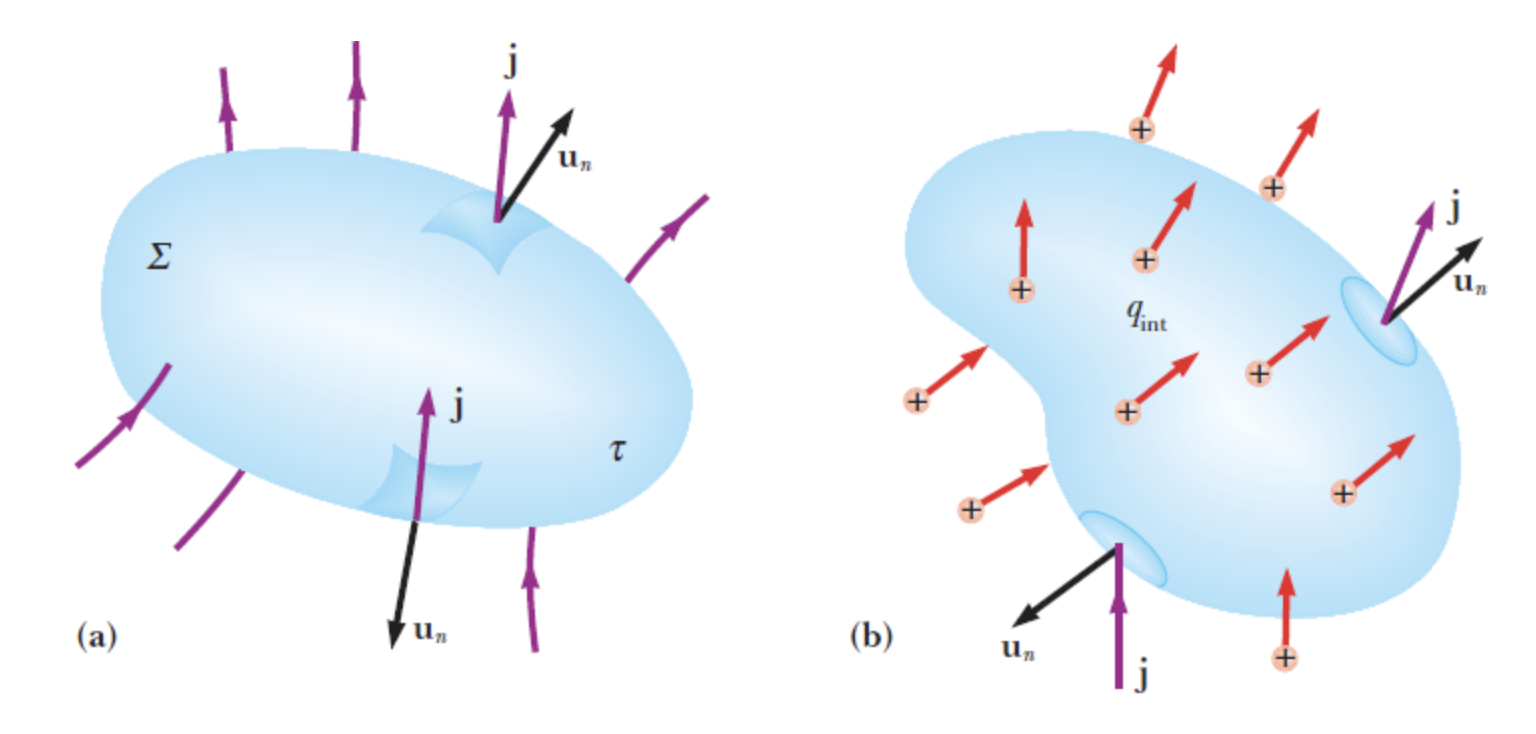
\includegraphics[width=0.75\linewidth]{figure/image39.png}
    \label{fig:chapter_12_1}
\end{figure}

Se la regione è sede di una corrente elettrica, definita dal vettore densità di corrente $\mathbf{J}$, la carica totale che passa nell'unità di tempo attraverso la superficie $\Sigma$ è data dal flusso di $\mathbf{J}$ attraverso $\Sigma$:

\begin{equation}
    I = \oint_{\Sigma} \mathbf{J} \cdot \mathbf{u}_n \ d\Sigma
\end{equation}

Il principio di conservazione della carica richiede che $I$, pari alla carica che attraversa $\Sigma$ nell'unità di tempo, sia eguale alla variazione nell'unità di tempo della carica complessiva $q_{\text{int}}$ contenuta all'interno di $\Sigma$

\begin{tcolorbox}[colback=yellow!10!white, colframe=orange!70!black, boxrule=0.8pt]
\begin{equation}
    I = \oint_{\Sigma} \mathbf{J} \cdot \mathbf{u}_n \ d\Sigma = - \frac{dq_{\text{int}}}{dt}
    \label{eq:principio_conservazione_carica}
\end{equation}
\end{tcolorbox}

\newpage

Un caso particolare e interessante si ha quando la carica interna interna non varia, per cui vale 

\begin{equation}
    \oint_{\Sigma} \mathbf{J} \cdot \mathbf{u}_n \ d\Sigma = 0
\end{equation}

Possiamo ricavare anche una forma locale della \ref{eq:principio_conservazione_carica}. Infatti possiamo scrivere questa può essere scritta come 

\begin{equation}
    \oint_{\Sigma} \mathbf{J} \cdot \mathbf{u}_n \ d\Sigma = - \int_{\tau} \frac{\partial \rho}{\partial t} \ d \tau
\end{equation}

Applicando il teorema della divergenza 

\begin{equation}
    \int_{\tau} \left( \nabla \cdot \mathbf{J} + \frac{\partial \rho}{\partial t} \right) d \tau = 0
\end{equation}

Dato che questo deve valere comunque di scelga il volume $\tau$ si deve avere 

\begin{tcolorbox}[colback=yellow!10!white, colframe=orange!70!black, boxrule=0.8pt]
\begin{equation} \label{eq:equazione_continuità}
    \nabla \cdot \mathbf{J} + \frac{\partial \rho}{\partial t} = 0
\end{equation}
\end{tcolorbox}

Questa \mkeyword{equazione di continuità della corrente} prende il nome di equazione di continuità della corrente ed esprime in modo dinamico la conservazione della carica elettrica.\\

In condizioni stazionarie si ha 

\begin{tcolorbox}[colback=yellow!10!white, colframe=orange!70!black, boxrule=0.8pt]
\begin{equation}
    \nabla \cdot \mathbf{J} = 0
\end{equation}
\end{tcolorbox}

\section{Conduttività elettrica e legge di Ohm}

Nella maggior parte delle sostanze, e in un ampio intervallo di intensità di campo elettrico, scopriamo che la densità di corrente è proporzionale all'intensità del campo elettrico che la causa. La relazione lineare tra densità di corrente e campo è espressa da

\begin{tcolorbox}[colback=yellow!10!white, colframe=orange!70!black, boxrule=0.8pt]
\begin{equation}
    \mathbf{J} = \sigma \ \mathbf{E}
    \label{eq:Legge_Ohm_conduzione}
\end{equation}
\end{tcolorbox}

Il \mkeyword{conduttività} fattore $\sigma$ è chiamato conduttività del materiale. Il suo valore dipende dal materiale in questione; è molto grande per i conduttori metallici, estremamente piccolo per i buoni isolanti. Può dipendere anche dallo stato fisico del materiale, ad esempio dalla sua temperatura.\\

La relazione \ref{eq:Legge_Ohm_conduzione} prende il nome di legge di Ohm della conduzione elettrica. Un'altra sua forma è la seguente

\begin{tcolorbox}[colback=yellow!10!white, colframe=orange!70!black, boxrule=0.8pt]
\begin{equation}
    \mathbf{E} = \rho \ \mathbf{J}
\end{equation}
\end{tcolorbox}

dove $\rho$ prende \mkeyword{resistività}il nome di resistività del conduttore . \footnote{Non andiamo ad approfondire oltre l'argomento, poiché trattato al corso di \emph{Laboratorio 2}}
